% ----------------------------------------------------------------------
\renewcommand{\CurrentProgressBarIs}{\FourOfFive}
% ----------------------------------------------------------------------
\begingroup
% \setbeamercolor{normal text}{bg=black}
\setbeamercolor{background canvas}{bg=mLightBrown!10}
\begin{frame}[t,plain]{4. Biomedical relation extraction (BioRE)}
\end{frame}
\endgroup
% ----------------------------------------------------------------------
\begingroup
\setbeamercolor{background canvas}{bg=mLightBrown!10}
\begin{frame}[t]{4. Biomedical relation extraction (BioRE)}

\centering
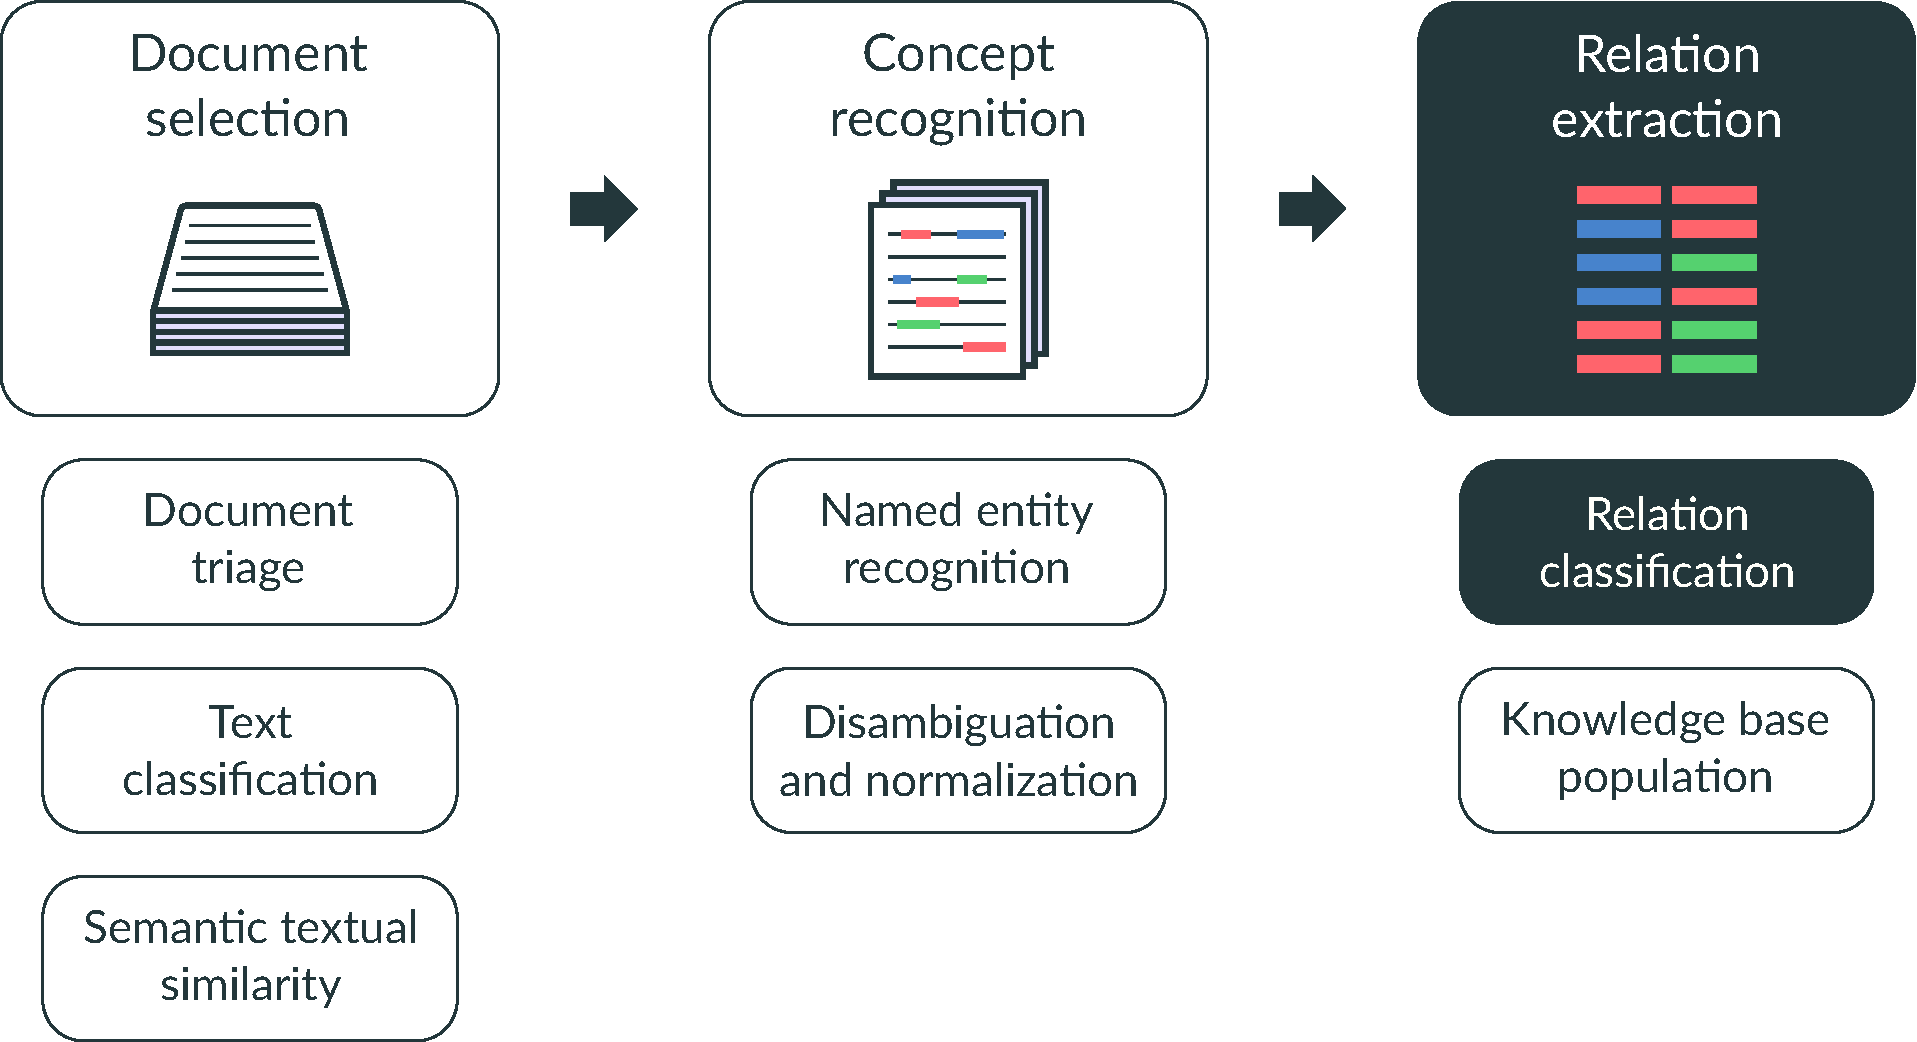
\includegraphics[width=0.80\textwidth]{img/biomedical-information-extraction/v3/007.pdf}%

\end{frame}
\endgroup
% ----------------------------------------------------------------------
\begin{frame}[t]{BioRE: Text mining chemical--protein interactions}

\vspace*{-5mm}

\small
\begin{itemize}
\setlength{\itemsep}{0.0pt}
\item ChemProt dataset (annotated PubMed abstracts)
\item Relations between chemical compounds (drugs) and genes (proteins)
\end{itemize}

% \vspace*{-2mm}
\vspace*{1mm}

% \small
% \footnotesize

\begin{center}
% \huge
% \LARGE
% \Large
% \normalsize
What a \chemical{chemical} does to a \protein{protein}?
\end{center}

% \vspace*{2mm}

% \small
\footnotesize
\centering

\begingroup
\renewcommand*{\arraystretch}{1.1}
\begin{tabular}{@{}lllll}
& & \blue{Activation} & &\\
& & \blue{Inhibition} & &\\
\chemical{Chemical} & \blue{$\xrightarrow{\hspace*{4mm}}$} & \blue{Agonist} & \blue{$\xrightarrow{\hspace*{4mm}}$} & \protein{Protein}\\[-2pt]
& & \blue{Antagonist} & & \\
& & \blue{Substrate} & & \\
\end{tabular}
\endgroup

\vspace*{3mm}
\RaggedRight
\fontsize{5pt}{6pt}\selectfont
\begin{tabular}{@{}l@{\hskip2pt}l}
Source: & Krallinger, Rabal, Akhondi, Pérez, Santamaría, Rodríguez \textit{et al.} (October 2017).\\
& \textit{Overview of the BioCreative VI chemical–protein interaction track}. BioCreative VI Workshop.\\
& \url{https://biocreative.bioinformatics.udel.edu/events/biocreative-vi/workshop/}
\end{tabular}

\end{frame}
% ----------------------------------------------------------------------
\begin{frame}[t]{BioRE: Text mining chemical--protein interactions}

\centering
\vspace*{-2mm}

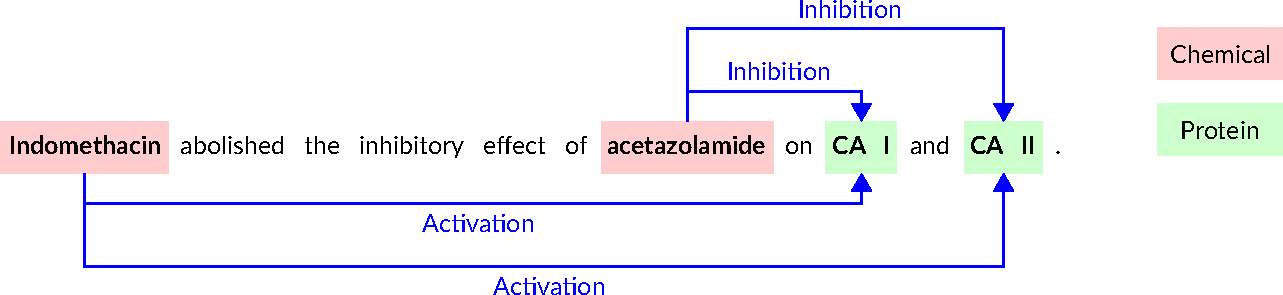
\includegraphics[width=0.95\textwidth]{img/chemprot-sentence/v2/001.pdf}%

\vspace*{-2mm}

% \footnotesize% 9pt
% \scriptsize% 8pt
% \tiny% 6pt
% \fontsize{5.75pt}{6.9pt}\selectfont
% \fontsize{5.5pt}{6.6pt}\selectfont
% \fontsize{5.25pt}{6.3pt}\selectfont
% \fontsize{5.2pt}{6.24pt}\selectfont
% \fontsize{5pt}{6pt}\selectfont

\newcommand{\minorscriptsize}{\fontsize{7.0pt}{8.4pt}\selectfont}
\newcommand{\minortiny}{\fontsize{5pt}{6pt}\selectfont}

\begin{columns}[t,totalwidth=\textwidth]

\begin{column}{0.10\textwidth}
\end{column}

\begin{column}{0.50\textwidth}

\begingroup\minorscriptsize
\textbf{\texttt{entities.tsv}}\\
\smallskip
\setlength{\fboxrule}{0.4pt}
\setlength{\fboxsep}{4pt}
% \small%
% \tiny%
\minortiny%
\fbox{%
\ttfamily%
\begin{tabular}{OllllllO}
...\\
\chemicaltext{8667211} & \chemicaltext{T1} & \chemicaltext{CHEMICAL} & \chemicaltext{1136} & \chemicaltext{1149} & \chemicaltext{acetazolamide}\\
...\\
\chemicaltext{8667211} & \chemicaltext{T12} & \chemicaltext{CHEMICAL} & \chemicaltext{1088} & \chemicaltext{1100} & \chemicaltext{Indomethacin}\\
\proteintext{8667211} & \proteintext{T13} & \proteintext{PROTEIN} & \proteintext{1153} & \proteintext{1157} & \proteintext{CA I}\\
\proteintext{8667211} & \proteintext{T14} & \proteintext{PROTEIN} & \proteintext{1162} & \proteintext{1167} & \proteintext{CA II}\\
...\\
\end{tabular}}
\endgroup

\end{column}

\begin{column}{0.40\textwidth}

\begingroup\minorscriptsize
\textbf{\texttt{relations.tsv}}\\
\smallskip
\setlength{\fboxrule}{0.4pt}
\setlength{\fboxsep}{4pt}
\minortiny%
\fbox{%
\ttfamily%
\begin{tabular}{OllllllO}
...\\
8667211 & \blue{CPR:3} & \chemicaltext{Arg1:T12} & \proteintext{Arg2:T13}\\
8667211 & \blue{CPR:3} & \chemicaltext{Arg1:T12} & \proteintext{Arg2:T14}\\
8667211 & \blue{CPR:4} & \chemicaltext{Arg1:T1}  & \proteintext{Arg2:T13}\\
8667211 & \blue{CPR:4} & \chemicaltext{Arg1:T1}  & \proteintext{Arg2:T14}\\
...\\
\end{tabular}}
\endgroup

\end{column}

\end{columns}

\vspace*{1mm}

\flushleft
\fontsize{5pt}{6pt}\selectfont
Source: ChemProt dataset (PMID 8667211)

\end{frame}
% ----------------------------------------------------------------------
\begin{frame}[t]{BioRE: ChemProt dataset statistics}

\centering

% \setlength{\fboxsep}{0pt}

% trim={<left> <lower> <right> <upper>}
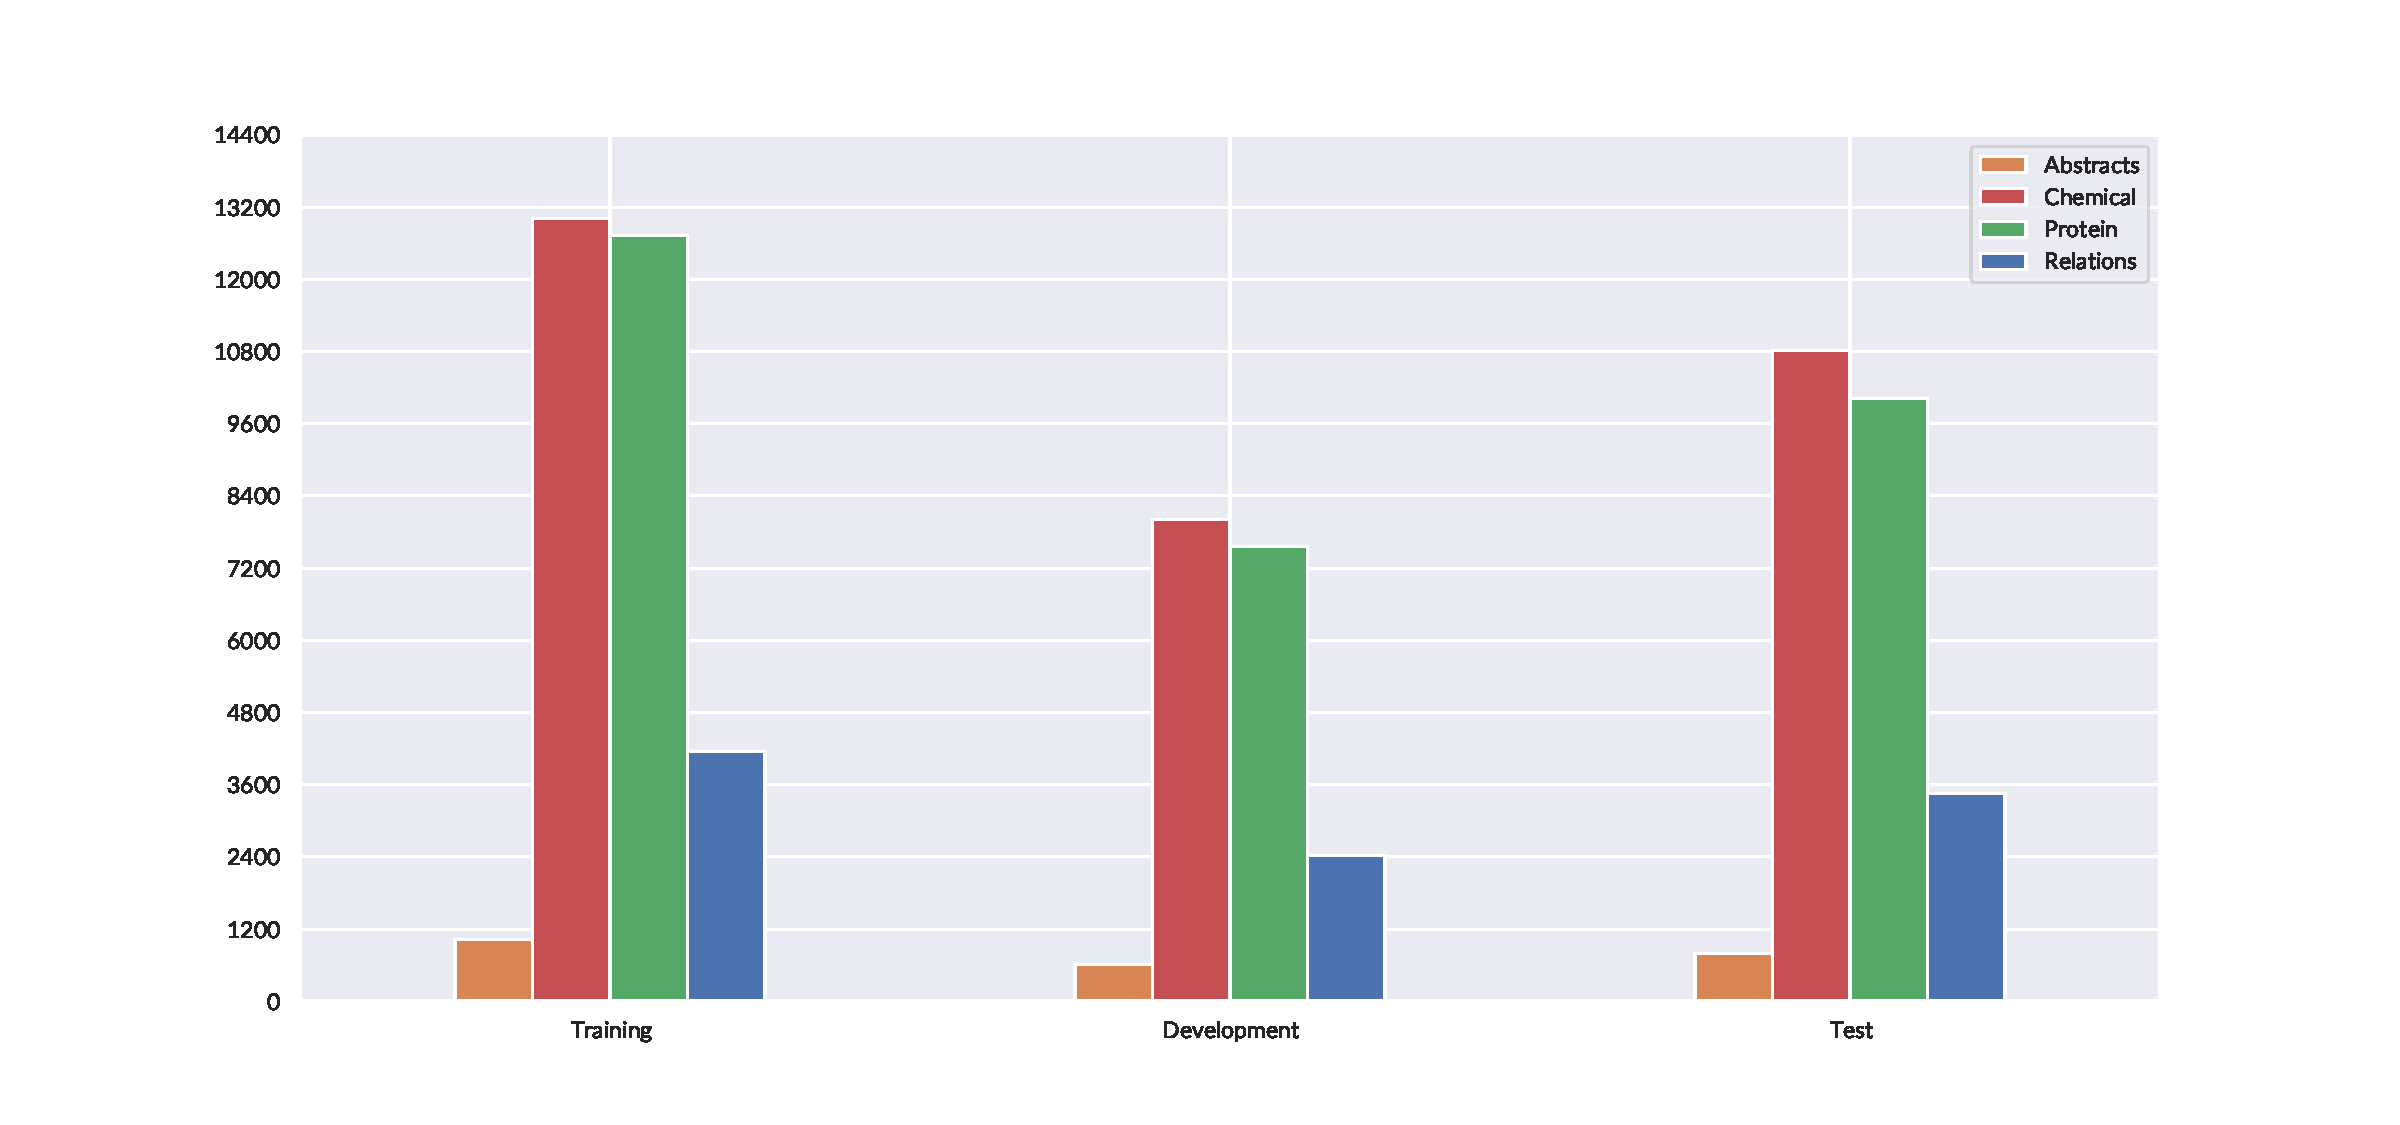
\includegraphics[width=\textwidth,trim={36mm 14mm 40mm 20mm},clip]{img/chemprot-dataset-statistics/v3/001.pdf}%

\end{frame}
% ----------------------------------------------------------------------
\begin{frame}[t]{BioRE: ChemProt relations statistics}
\centering
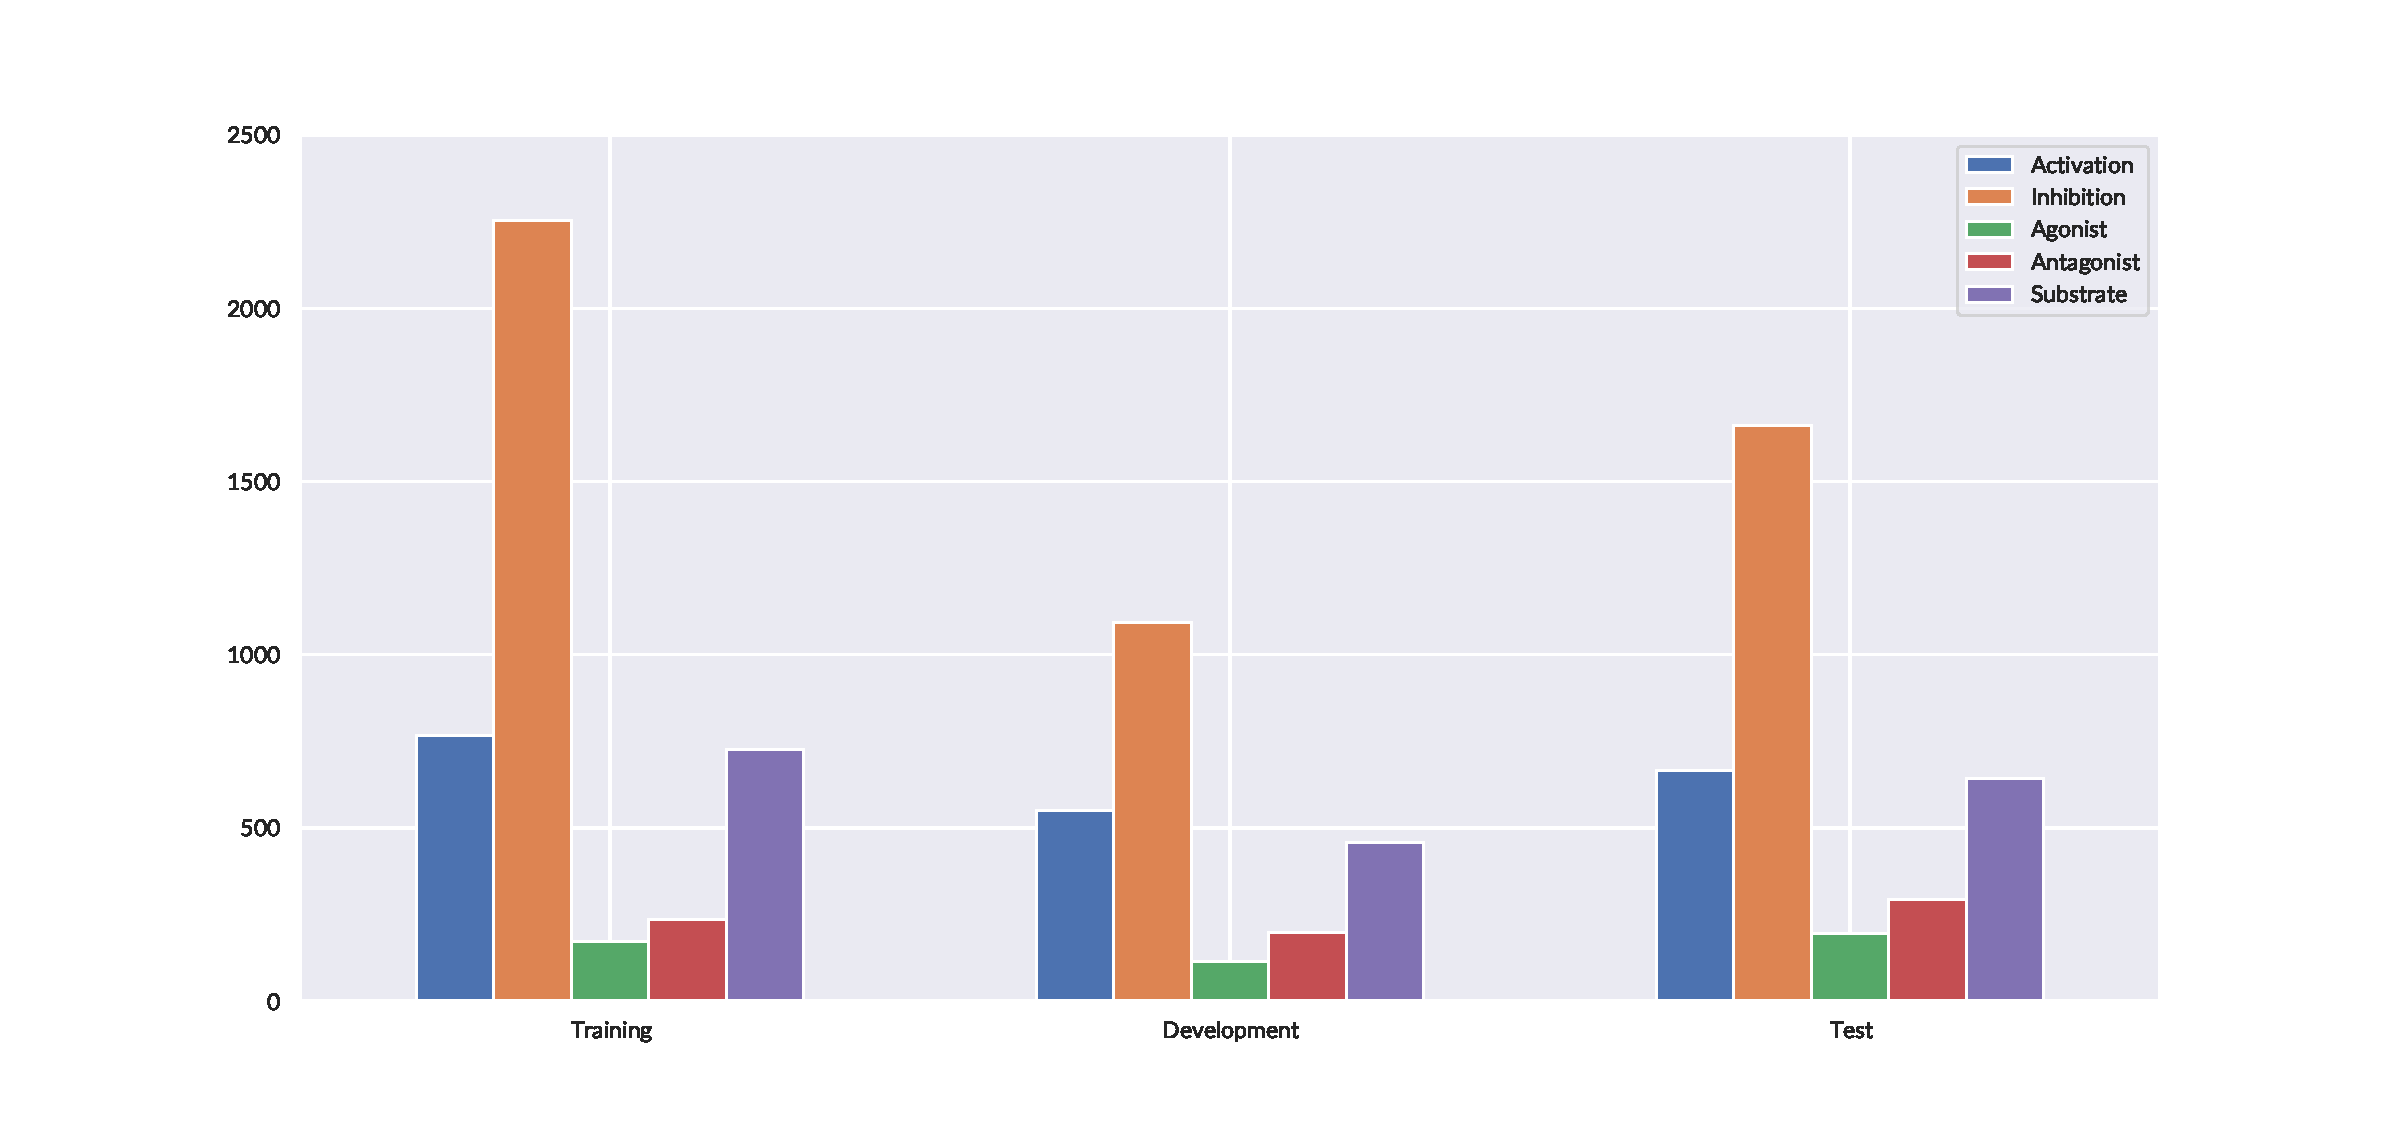
\includegraphics[width=\textwidth,trim={36mm 14mm 40mm 20mm},clip]{img/chemprot-relations-statistics/v2/001.pdf}%
\end{frame}
% ----------------------------------------------------------------------
\begin{frame}[t]{BioRE: ChemProt --- Text pre-processing}

\begin{tikzpicture}[overlay]\fontsize{5.6}{6.72}\selectfont
\node[anchor=west] at (-0.08,  0.30) {\textbf{Turku Event Extraction System}};
\node[anchor=west] at (-0.08, -0.05) {%
\raisebox{-0.35\baselineskip}{
\includegraphics[height=1.10\baselineskip]{img/logos/github.pdf}}~%
\href{https://github.com/jbjorne/TEES}{\texttt{jbjorne/TEES}}};
\end{tikzpicture}

\centering

% \vspace*{-2mm}
\vspace*{-7mm}

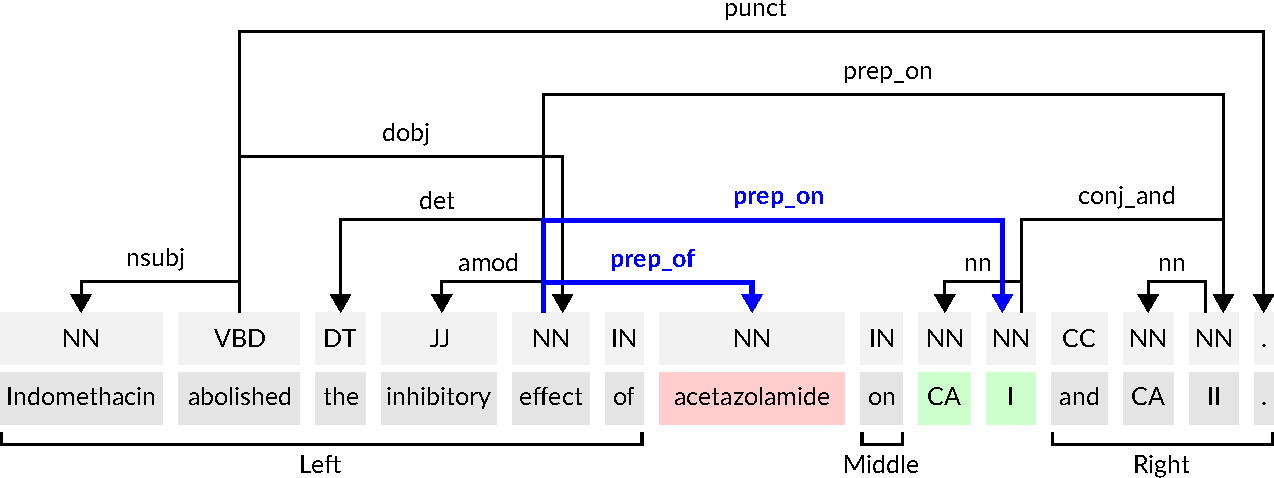
\includegraphics[width=0.8\textwidth]{img/chemprot-sample/v1/005.pdf}%

% \bigskip
\medskip

{\scriptsize\texttt{CPR:4/8667211\_7\_T1\_T13.txt}}

\setlength{\fboxrule}{0.5pt}
\setlength{\fboxsep}{4pt}
\fbox{%
\ttfamily%
\fontsize{5.6}{6.72}\selectfont%
%\tiny%
\begin{tabular}{Ol@{\hskip6mm}lO}
Shortest dependency path & \chemicaltext{chemical}|NN|\blue{prep\_of}|effect|NN|\blue{prep\_on}|\proteintext{protein}|NN|\\
Chemical left text & Indomethacin|NN|nsubj|abolished|VBD||the|DT|det|inhibitory|JJ|amod|effect|NN|dobj|of|IN|\\
Chemical right text & on|IN|\\
Protein left text & on|IN|\\
Protein right text & and|CC||CA|NN|nn|II|NN|prep\_on|.|.|punct\\
\end{tabular}
}

\end{frame}
% ----------------------------------------------------------------------
\begin{frame}[t]{BioRE: ChemProt --- Neural network structure}

\centering

% \vspace*{-2mm}

% \hspace*{16mm}
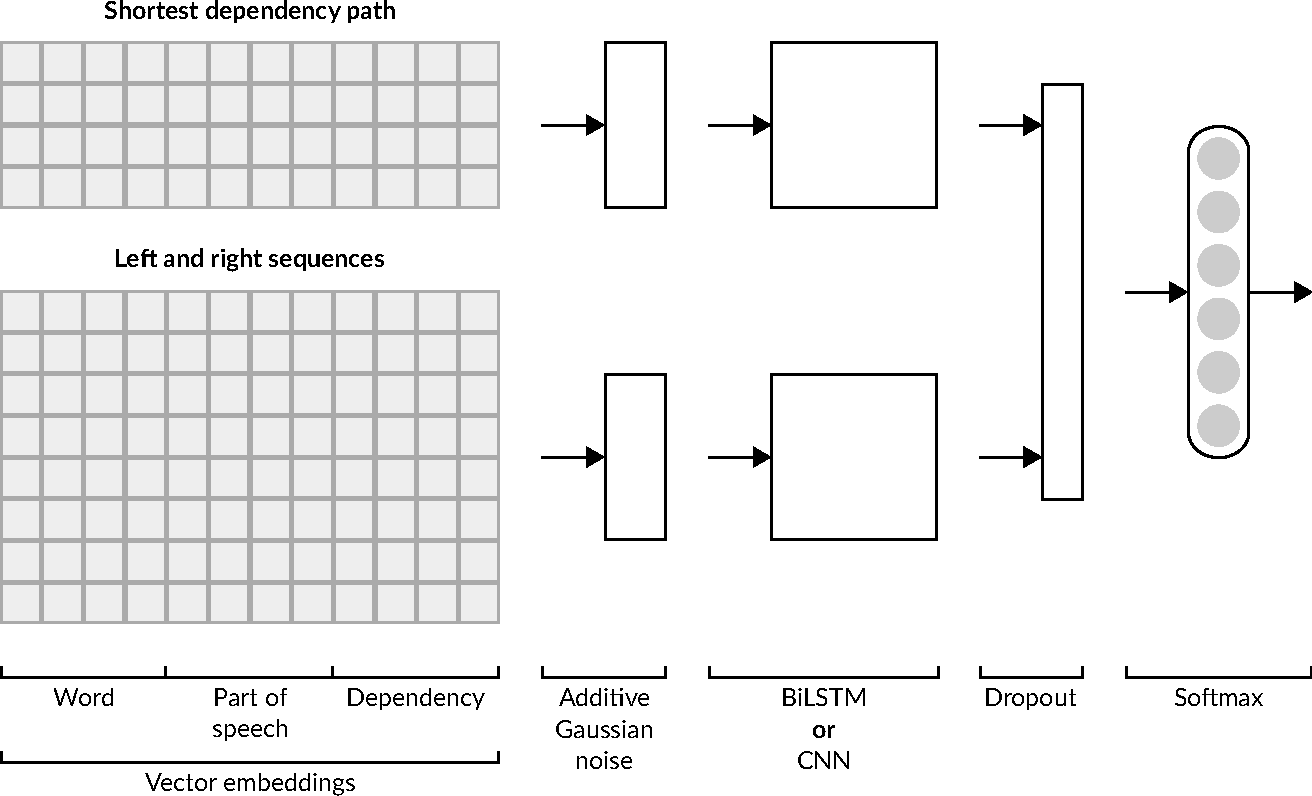
\includegraphics[width=0.75\textwidth]{img/chemprot-nn/v3/001.pdf}%

\end{frame}
% ----------------------------------------------------------------------
\begin{frame}[t]{BioRE: ChemProt --- Parameters and additional techniques}

% \centering

\vspace*{-2mm}

\begin{columns}[t,totalwidth=\textwidth]

% \begin{column}{0.05\textwidth}
% \end{column}

\begin{column}{0.50\textwidth}

% \scriptsize
\tiny
\renewcommand*{\arraystretch}{1.1}
\begin{tabular}{l@{\hskip4mm}l}
\toprule
Gaussian noise standard deviation & 0.01\\
LSTM units & 128\\
LSTM recurrent dropout & 0.4\\
LSTM dropout & 0.4\\
Convolution filters & 64\\
Convolution window sizes & [3, 4, 5]\\
Dropout rate & 0.4\\
\midrule
Optimizer & RMSprop\\
Loss & Categorical cross entropy\\
\midrule
Batch size & 128\\
Maximum number of epochs & 500\\
Early stopping patience & 30\\
Early stopping monitor & Validation micro F1-score\\
Validation split & 0.3\\
\bottomrule
\end{tabular}

\end{column}

% \vspace*{-5mm}
% \vspace*{-4mm}

\begin{column}{0.50\textwidth}

\vspace*{-2mm}

% \normalsize % 11pt
\fontsize{10.25pt}{12.30pt}\selectfont
% \small % 10pt
% \footnotesize
\begin{itemize}
\setlength{\itemsep}{20.0pt}
\item Averaging of three simulations (different random states)
\item Balancing between precision and recall (maximize F1-score)
\item Additional training data from BioGRID (distant supervision)
\end{itemize}

\end{column}

\end{columns}

\end{frame}
% ----------------------------------------------------------------------
\begin{frame}[t]{BioRE: ChemProt --- F1-score on \textit{development} set}

\centering
\scriptsize

% \vspace*{-2mm}

\renewcommand*{\arraystretch}{0.8}
\begin{tabular}{lllllll}
% \toprule
(WS, PS, DS) & Features & \multicolumn{1}{l}{Model} & W & W + P & \alert{W + D} & W + P + D\\
\midrule
\multirow{6}{*}[-5pt]{(300\textsuperscript{a}, 100, 100)} & \multirow{2}{*}{SDP} & BiLSTM & 0.6161 & 0.6002 & \textbf{0.6473} & 0.6310\\
& & CNN & 0.5642 & 0.5782 & \textbf{0.6141} & 0.6092\\
\cmidrule{2-7}
& \multirow{2}{*}{LR} & BiLSTM & 0.5135 & 0.5133 & 0.5209 & \textbf{0.5227}\\
& & CNN & 0.4293 & \textbf{0.4576} & 0.4321 & 0.4216\\
\cmidrule{2-7}
& \multirow{2}{*}{SDP + LR} & BiLSTM & 0.5914 & 0.5812 & \textbf{0.6036} & 0.6015\\
& & CNN & 0.5572 & 0.5618 & 0.5672 & \textbf{0.5819}\\
\cmidrule{1-7}
\alert{\multirow{6}{*}[-5pt]{(200\textsuperscript{b}, 50, 50)}} & \alert{\multirow{2}{*}{SDP}} & \alert{BiLSTM} & 0.6229 & 0.6192 & \alert{\textbf{0.6496}} & 0.6453\\
& & CNN & 0.5804 & 0.5841 & \textbf{0.6259} & 0.6205\\
\cmidrule{2-7}
& \multirow{2}{*}{LR} & BiLSTM & 0.5030 & \textbf{0.5158} & 0.5060 & 0.4849\\
& & CNN & \textbf{0.4813} & 0.4504 & 0.4201 & 0.4291\\
\cmidrule{2-7}
& \multirow{2}{*}{SDP + LR} & BiLSTM & 0.5943 & 0.5993 & \textbf{0.6126} & 0.5824\\
& & CNN & 0.5690 & 0.5440 & \textbf{0.5760} & 0.5605\\
%\bottomrule
\midrule\addlinespace[4pt]
\multicolumn{7}{l}{\tiny\textsuperscript{a} Our PubMed-based word2vec vectors}\\
\multicolumn{7}{l}{\tiny\textsuperscript{b} BioWordVec fastText vectors by Chen \textit{et al.} (2019)}
\end{tabular}

\end{frame}
% ----------------------------------------------------------------------
\begin{frame}[t]{BioRE: ChemProt --- F1-score on \textit{development} and \textit{test} sets}

\centering
\scriptsize

% \vspace*{-2mm}

\renewcommand*{\arraystretch}{1.1}

\begin{tabular}{lllll}
% \toprule
\multicolumn{1}{l}{(WS, PS, DS)} & \multicolumn{1}{l}{} & & Development & Test\\
\midrule
\multirow{2}{*}{(300\textsuperscript{a}, 100, 100)} & \multirow{2}{*}{Baseline} & BiLSTM & 0.6473 & 0.6182\\
& & CNN & 0.6141 & 0.5932\\
\midrule
\alert{\multirow{6}{*}{(200\textsuperscript{b}, 50, 50)}} & \alert{\multirow{2}{*}{Baseline}} & \alert{BiLSTM} & \alert{\textbf{0.6496}} & \alert{0.6306}\\
& & CNN & 0.6259 & 0.5959\\
\cmidrule{2-5}
& \multirow{2}{*}{BioGRID} & BiLSTM & 0.5871 & 0.5964\\
& & CNN & 0.5774 & 0.5701\\
\cmidrule{2-5}
& \multirow{2}{*}{No validation\textsuperscript{c}} & BiLSTM & 0.6443 & \textbf{0.6360}\\
& & CNN & 0.5547 & 0.5586\\
% \bottomrule
\midrule\addlinespace[1pt]
\multicolumn{5}{l}{\tiny\textsuperscript{a} Our PubMed-based word2vec vectors}\\[-4pt]
\multicolumn{5}{l}{\tiny\textsuperscript{b} BioWordVec fastText vectors by Chen \textit{et al.} (2019)}\\[-4pt]
\multicolumn{5}{l}{\tiny\textsuperscript{c} Model trained during 500 epochs (without monitoring)}
\end{tabular}

\end{frame}
% ----------------------------------------------------------------------
\begin{frame}[t]{BioRE: ChemProt --- Confusion matrix on \textit{test} set}

\centering
\tiny
% \scriptsize

\vspace*{-2mm}
% \vspace*{-4mm}
% \vspace*{-6mm}

\newcommand{\z}{\hphantom{0}}

\renewcommand*{\arraystretch}{1.4}

\begin{tabular}{E{14mm}R{12mm}R{12mm}R{12mm}R{12mm}R{12mm}R{12mm}R{12mm}}

Predicted & \multicolumn{6}{c}{Gold standard} &\\

\cmidrule(r{2em}){1-1}\cmidrule{2-7}

& Negative & CPR:3 & CPR:4 & CPR:5 & CPR:6 & CPR:9 & Sum\\[-4pt]
& & Activation & Inhibition & Agonist & Antagonist & Substrate &\\

Negative & & \cellcolor[RGB]{245,224,82}238 & \cellcolor[RGB]{245,224,82}\z524 & \cellcolor[RGB]{245,224,82}\z97 & \cellcolor[RGB]{245,224,82}124 & \cellcolor[RGB]{245,224,82}341 & 1324\\
Activation & \cellcolor[RGB]{255,133,155}263 & \cellcolor[RGB]{51,204,77}382 & \cellcolor[RGB]{245,224,82}\z\z19 & \cellcolor[RGB]{245,224,82}\z\z5 & \cellcolor[RGB]{245,224,82}\z\z0 & \cellcolor[RGB]{245,224,82}\z\z0 & \z669\\
Inhibition & \cellcolor[RGB]{255,133,155}401 & \cellcolor[RGB]{245,224,82}\z45 & \cellcolor[RGB]{51,204,77}1107 & \cellcolor[RGB]{245,224,82}\z14 & \cellcolor[RGB]{245,224,82}\z\z2 & \cellcolor[RGB]{245,224,82}\z\z2 & 1571\\
Agonist & \cellcolor[RGB]{255,133,155}\z45 & \cellcolor[RGB]{245,224,82}\z\z0 & \cellcolor[RGB]{245,224,82}\z\z\z2 & \cellcolor[RGB]{51,204,77}\z79 & \cellcolor[RGB]{245,224,82}\z\z6 & \cellcolor[RGB]{245,224,82}\z\z0 & \z132\\
Antagonist & \cellcolor[RGB]{255,133,155}\z56 & \cellcolor[RGB]{245,224,82}\z\z0 & \cellcolor[RGB]{245,224,82}\z\z\z1 & \cellcolor[RGB]{245,224,82}\z\z0 & \cellcolor[RGB]{51,204,77}161 & \cellcolor[RGB]{245,224,82}\z\z0 & \z218\\
Substrate & \cellcolor[RGB]{255,133,155}185 & \cellcolor[RGB]{245,224,82}\z\z0 & \cellcolor[RGB]{245,224,82}\z\z\z8 & \cellcolor[RGB]{245,224,82}\z\z0 & \cellcolor[RGB]{245,224,82}\z\z0 & \cellcolor[RGB]{51,204,77}301 & \z494\\
Sum & 950 & \cellcolor[RGB]{133,255,255}665 & \cellcolor[RGB]{133,255,255}1661 & \cellcolor[RGB]{133,255,255}195 & \cellcolor[RGB]{133,255,255}293 & \cellcolor[RGB]{133,255,255}644 &\\

\multicolumn{8}{c}{}\\

\arrayrulecolor{white}
% \multicolumn{2}{l}{} & \multicolumn{2}{l}{\hskip40pt Total gold standard relations} & 3458 & \multicolumn{2}{r}{\cellcolor[RGB]{133,255,255}} &\\
% \hline\hline
% \multicolumn{2}{l}{} & \multicolumn{2}{l}{\hskip40pt Total predicted relations} & 2980 & \multicolumn{1}{r}{\cellcolor[RGB]{51,204,77}} & \multicolumn{1}{r}{\cellcolor[RGB]{255,133,155}} &\\
% \hline\hline
\multicolumn{2}{l}{} & \multicolumn{2}{l}{\hskip40pt True positives} & 2030 & \multicolumn{2}{r}{\cellcolor[RGB]{51,204,77}} &\\
\hline\hline
\multicolumn{2}{l}{} & \multicolumn{2}{l}{\hskip40pt False negatives} & 1428 & \multicolumn{2}{r}{\cellcolor[RGB]{245,224,82}} &\\
\hline\hline
\multicolumn{2}{l}{} & \multicolumn{2}{l}{\hskip40pt False positives} & \z950 & \multicolumn{2}{r}{\cellcolor[RGB]{255,133,155}} &\\

\end{tabular}

\end{frame}
% ----------------------------------------------------------------------
\begin{frame}[t]{BioRE: ChemProt --- Error analysis}

\centering
\scriptsize

% \vspace*{-2mm}

% Present only a few examples.
% Otherwise it may become too heavy to read.

\renewcommand*{\arraystretch}{1.2}
\begin{tabular}{E{60mm}E{30mm}E{15mm}E{15mm}}
% \toprule
Sentence & Words in the SDP & Predicted & Correct\\
\midrule
The \blue{introduction} of the \chemicaltext{amino} \blue{group} \blue{resulted} in not only improved water solubility but also enhanced \proteintext{TLR7} \alert{agonistic} \blue{activity}. & group introduction resulted activity & Activation & Agonist\\
\midrule
% Our work shows that \chemicaltext{sulfonylureas} and glinides additionally bind to PPARgamma and \blue{exhibit} \proteintext{PPARgamma} \alert<4>{agonistic} \blue{activity}. & exhibit activity & Inhibition & Agonist\pause\pause\\
% \midrule
In guinea pigs, \alert{antagonist actions} of \chemicaltext{yohimbine} at \proteintext{5-HT(1B)} \blue{receptors} are revealed by blockade of hypothermia evoked by the 5-HT(1B) agonist, GR46,611. & receptors & Agonist & Antagonist\\
\midrule
% Impaired expression of the uncoupling protein-3 gene in skeletal muscle during lactation: fibrates and \chemicaltext{troglitazone} \blue{reverse} lactation-induced \blue{downregulation} of the \proteintext{uncoupling protein-3} \blue{gene}. & reverse \alert<8>{downregulation} gene & Inhibition & Activation\pause\pause\\
% \midrule
\chemicaltext{Geldanamycin} also \blue{disrupts} the T-cell receptor-mediated \blue{activation} of \proteintext{nuclear factor of activated T-cells} (NF-AT). & \leavevmode\alert{disrupts activation} & Activation & Inhibition\\
% \midrule
% Blockade of \chemicaltext{LTC4} \blue{synthesis} \blue{caused} by additive \blue{inhibition} of \proteintext{gIV-PLA2} \blue{phosphorylation}: Effect of salmeterol and PDE4 inhibition in human eosinophils. & synthesis caused \alert<6>{inhibition} phosphorylation & Inhibition & Substrate\pause
% \bottomrule
\end{tabular}

\end{frame}
% ----------------------------------------------------------------------
\begin{frame}[t]{BioRE: ChemProt participating teams (F1-score results)}

\centering
\tiny

% \vspace*{-2mm}

\renewcommand*{\arraystretch}{1.3}
\begin{tabular}{rllrr}
% \toprule
Rank & Authors & Methods & Challenge & Post-challenge\\
% \midrule
\cmidrule{1-5}
1 & Peng, Rios, Kavuluru, and Lu & SVM, CNN and RNN & \textbf{0.6410}\\
2 & Corbett and Boyle & RNN and CNN & 0.6141 & 0.6258\\
3 & Mehryary, Björne, Salakoski, and Ginter & SVM and RNN & 0.6099 & 0.6310\\
4 & Lim and Kang & Tree-structured RNN & 0.5853 & 0.6410\\
5 & Lung, He, Zhao, Yu, and Zhang & Traditional ML & 0.5671 &\\
\alert{6} & \alert{Antunes and Matos} & \alert{RNN and CNN} & \alert{0.5181} & \alert{0.6306}\\
7 & Liu, Shen, Elayavilli, Wang \textit{et al.} & CNN and attention-based RNN & 0.4948 & 0.5270\\
8 & Verga and McCallum & Bi-affine attention network & 0.4582 &\\
9 & Wang, Yang, Xing, Wu, and Song & RNN & 0.3839 &\\
10 & Tripodi, Boguslav, Hailu, and Hunter & Traditional ML and neural networks & 0.3700 &\\
11 & Warikoo, Chang, and Hsu & Tree kernel & 0.3092 & 0.3654\\
12 & Sun & & 0.2195 &\\
13 & Yüksel, Öztürk, Ozkirimli, and Özgür & CNN & 0.1864 &\\
% \bottomrule
\end{tabular}

\end{frame}
% ----------------------------------------------------------------------
